\documentclass[11pt,a4paper]{article}

\usepackage[margin=2.0cm]{geometry}
\usepackage[T1]{fontenc}
\usepackage{amsmath,amssymb}
\usepackage{graphicx}
\usepackage{booktabs}
\usepackage{subcaption}
\usepackage{xcolor}
\usepackage{float}
\usepackage[numbers,sort&compress]{natbib}
\usepackage[hidelinks]{hyperref}
\usepackage{titlesec}

\titlespacing*{\section}{0pt}{1.4ex}{0.6ex}
\titlespacing*{\subsection}{0pt}{1.0ex}{0.4ex}
\titlespacing*{\paragraph}{0pt}{0.6ex}{0.8em}
\setlength{\parskip}{0.35ex}
\graphicspath{{figures/}}

\title{\vspace{-2.2em}\textbf{Quantization for Efficient LLM Inference:\\
A Quality--Memory--Speed Study of Qwen2.5-7B-Instruct}}
\author{Hubert Michalski \quad Przemys{\l}aw Fuchs\\[2pt]
\small University of Warsaw \quad \{hm438596, pf438429\}@students.mimuw.edu.pl}
\date{}

\begin{document}
\maketitle
\vspace{-1.8em}

\begin{abstract}
\noindent
Quantization lets large language models run on cheaper hardware, but a smaller
model is not automatically a better one: it may lose accuracy, become
\emph{slower} in some runtimes, or save only disk rather than compute memory. We
study these trade-offs for a single 7B-class instruction model,
\textbf{Qwen2.5-7B-Instruct}, comparing a \texttt{bf16} baseline against four
post-training quantization variants (8-bit \texttt{LLM.int8()}, 4-bit
\texttt{NF4}, and official 4-bit \texttt{GPTQ} and \texttt{AWQ}) on four
capability benchmarks (MMLU, GSM8K, HumanEval, IFEval) and a battery of
efficiency measurements, all on a single RTX~4090. We find that \textbf{4-bit
GPTQ/AWQ give the best overall trade-off}---they are the only variants that cut
both disk \emph{and} GPU memory while staying close to baseline speed, at a
graceful ${\sim}1.5$~pt MMLU cost. Two counter-intuitive results stand out:
\texttt{LLM.int8()} is the \emph{slowest} variant ($5\times$ slower decode than
\texttt{bf16}) and saves no disk, and \texttt{NF4} saves memory but is also
slower than \texttt{bf16}---confirming that quantization is primarily a
\emph{memory} technique, not a speed one. We additionally implement and run four
catalogued extensions on the box (JudgeBench meta-evaluation, W8A8/SmoothQuant
self-quantization, a quantized KV cache, and QLoRA recovery), which sharpen the
``memory vs.\ speed'' story.
\end{abstract}

\section{Introduction and Research Questions}

Many LLMs are too expensive to serve in full precision, and post-training
quantization is the standard remedy. The literature offers several practical
methods: \texttt{LLM.int8()} \citep{llmint8} for 8-bit weights with
mixed-precision outlier handling; \texttt{GPTQ} \citep{gptq} and \texttt{AWQ}
\citep{awq}, which use a small calibration set to push weights to 4 bits;
\texttt{SmoothQuant} \citep{smoothquant} for 8-bit weights \emph{and}
activations; the \texttt{NF4} data type from \texttt{QLoRA} \citep{qlora} for
4-bit storage in the \texttt{bitsandbytes} ecosystem; and KV-cache quantization
such as KIVI \citep{kivi} for long-context inference. These methods are not
automatically beneficial---the same 4-bit model can be smaller yet slower, or
degrade unevenly across capabilities---so the practical trade-off is exactly
what we measure. We organise the study around four questions from our proposal:

\begin{enumerate}\itemsep1pt
\item[\textbf{RQ1}] Which method gives the best \emph{quality--memory--speed}
  trade-off for a 7B-class instruction LLM?
\item[\textbf{RQ2}] Are some \emph{capabilities} (reasoning, coding, QA,
  instruction following) more sensitive to quantization than others?
\item[\textbf{RQ3}] Does quantization improve real \emph{inference speed}, or
  mainly reduce \emph{memory}?
\item[\textbf{RQ4}] \emph{(optional)} Can light QLoRA-style adaptation recover
  quality lost after 4-bit quantization?
\end{enumerate}

Our core study is the proposal's ``minimal successful version'' (one model, five
variants, four benchmarks, full efficiency profiling); we then implement the
catalogued extensions as a gated code layer and run the four that fit our GPU
budget.

\section{Experimental Setup}

\paragraph{Model and variants.} All experiments use
\textbf{Qwen2.5-7B-Instruct} \citep{qwen25} at a pinned commit, run on a single
on-demand \textbf{RTX~4090 (24\,GB, sm\_89)}; every variant---including the
\texttt{bf16} baseline---runs on the same homogeneous GPU, so the speed
comparison is apples-to-apples with no cross-hardware caveat. Table~\ref{tab:variants}
lists the five core variants. \texttt{LLM.int8()} and \texttt{NF4} quantize the
baseline weights at load time (so their \emph{disk} footprint is the full
\texttt{bf16} checkpoint); GPTQ/AWQ are official pre-quantized 4-bit checkpoints
served by the \texttt{gptqmodel} Marlin kernels through \texttt{optimum}.

\paragraph{Benchmarks and protocol.} Quality is measured with the
EleutherAI \texttt{lm-evaluation-harness} \citep{lmeval}: MMLU \citep{mmlu}
(accuracy, aggregated weighted over its 57 subjects), GSM8K \citep{gsm8k}
(exact-match under \emph{flexible} extraction---the strict-match number is a
formatting artefact for instruct models), HumanEval \citep{humaneval}
(\texttt{pass@1}, with code execution), and IFEval \citep{ifeval}
(prompt-level strict accuracy). Decoding is greedy and deterministic
(\texttt{do\_sample=False} at load \emph{and} generation); MMLU/GSM8K use the
chat template with 5-shot multi-turn prompting, HumanEval/IFEval are 0-shot.
Efficiency is profiled separately (\S\ref{sec:eff}): the model is loaded once,
then we measure disk size, load/generate peak VRAM, prefill and decode
throughput at short/medium/long prompts (128/1024/4096 tokens), and the maximum
batch size before OOM.

\begin{table}[H]
\centering\small
\begin{tabular}{llll}
\toprule
Variant & Method & Precision & Source \\
\midrule
\texttt{bf16}          & half-precision baseline                 & W16     & reference \\
\texttt{bnb-int8}      & \texttt{LLM.int8()} \citep{llmint8}      & W8 (load-time)  & \texttt{bitsandbytes} \\
\texttt{bnb-nf4}       & NF4 + double-quant \citep{qlora}         & W4 (load-time)  & \texttt{bitsandbytes} \\
\texttt{gptq-official} & GPTQ \citep{gptq}                        & W4 (g128)       & official Qwen ckpt \\
\texttt{awq-official}  & AWQ \citep{awq}                          & W4 (g128)       & official Qwen ckpt \\
\bottomrule
\end{tabular}
\caption{The five core variants. ``Load-time'' means the disk checkpoint is the
full \texttt{bf16} model, quantized in memory during loading.}
\label{tab:variants}
\end{table}

\section{Results}

\subsection{Quality: capability sensitivity (RQ2)}

Table~\ref{tab:quality} and Figure~\ref{fig:quality} report quality across the
four benchmarks. The headline is that \textbf{quantization is remarkably benign
for quality at 7B}: every 4-bit variant stays within ${\sim}1.5$~points of the
\texttt{bf16} baseline on MMLU and GSM8K. Capability sensitivity is uneven,
answering RQ2:

\begin{itemize}\itemsep1pt
\item \textbf{Knowledge/QA and math are nearly lossless.} MMLU drops only
  $73.6\!\to\!72.1$--$72.6$ (4-bit) and is essentially unchanged for 8-bit
  ($73.4$); GSM8K stays at $83$--$84.5\%$ throughout.
\item \textbf{Coding (HumanEval) is the most quantization-sensitive capability.}
  It falls $84.1\!\to\!79.9$ for \texttt{bnb-int8} ($-4.2$\,pt, the single
  largest drop) and to ${\sim}81$ for the 4-bit methods.
\item \textbf{Instruction following (IFEval)} degrades mildly ($71.3\!\to\!69$--$71$);
  interestingly \texttt{bnb-nf4} ($71.0$) essentially ties the baseline.
\end{itemize}
8-bit is close to lossless on knowledge/math but, surprisingly, gives the
\emph{worst} HumanEval of all variants---so ``more bits'' does not uniformly mean
``higher quality.''

\begin{table}[H]
\centering\small
\begin{tabular}{lccccc}
\toprule
Variant & MMLU & GSM8K & HumanEval & IFEval & Mean \\
        & (acc) & (flex.\ EM) & (pass@1) & (strict) & \\
\midrule
\texttt{bf16}          & \textbf{73.6}\,$\pm$0.4 & \textbf{84.5} & \textbf{84.1} & \textbf{71.3} & \textbf{78.4} \\
\texttt{bnb-int8}      & 73.4 & 84.4 & 79.9 & 69.3 & 76.8 \\
\texttt{bnb-nf4}       & 72.6 & 83.6 & 81.7 & 71.0 & 77.2 \\
\texttt{gptq-official} & 72.1 & 83.2 & 81.1 & 70.2 & 76.7 \\
\texttt{awq-official}  & 72.2 & 84.3 & 81.1 & 69.9 & 76.9 \\
\bottomrule
\end{tabular}
\caption{Quality (\%). MMLU is weighted over 57 subjects ($\pm$ standard error
shown); GSM8K uses flexible-extract exact-match. Best per column in bold.}
\label{tab:quality}
\end{table}

\begin{figure}[H]
\centering
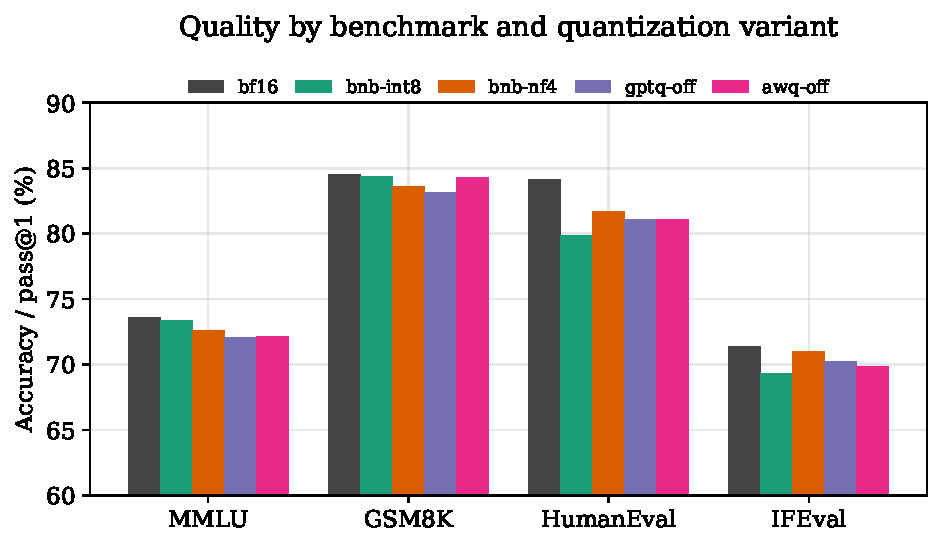
\includegraphics[width=0.92\linewidth]{fig_quality.pdf}
\caption{Quality by benchmark and variant. The 4-bit methods cluster tightly;
HumanEval (coding) shows the widest spread, with \texttt{bnb-int8} the most
degraded.}
\label{fig:quality}
\end{figure}

\subsection{Efficiency: memory vs.\ speed (RQ3)}
\label{sec:eff}

The efficiency profile (Table~\ref{tab:eff}, Figure~\ref{fig:eff}) gives the
clearest and most surprising findings, and directly answers RQ3:
\textbf{quantization is primarily a memory technique, not a speed one.}

\begin{itemize}\itemsep1pt
\item \textbf{\texttt{LLM.int8()} is the slowest variant.} Its decode throughput
  collapses to $7.2$~tok/s---$5\times$ slower than \texttt{bf16}'s $37.0$---
  because of the mixed-precision outlier decomposition, and it saves \emph{no}
  disk (it is the full \texttt{bf16} checkpoint). It is the worst of both worlds
  on the speed/disk axes.
\item \textbf{\texttt{NF4} is memory-not-speed.} It cuts generate VRAM to
  $5.95$\,GiB (from $14.96$) and doubles the max batch to 32, but decodes at
  $16.9$~tok/s---still \emph{below} \texttt{bf16}.
\item \textbf{GPTQ/AWQ are the only ``free lunch.''} They cut disk to $5.19$\,GiB
  (a genuine $2.7\times$ on-disk shrink), generate VRAM to ${\sim}5.95$\,GiB,
  raise the max batch to 32, \emph{and} keep decode near baseline at
  ${\sim}28$~tok/s---the only variants that improve memory without paying a large
  speed penalty.
\item \textbf{Prefill is unaffected} (${\sim}9.2$--$9.7$\,k tok/s for all
  variants): quantization touches the memory-bound decode phase, not the
  compute-bound prefill.
\end{itemize}

\begin{table}[H]
\centering\small
\begin{tabular}{lcccccc}
\toprule
Variant & Disk & Gen.\ VRAM & Max & Decode & Prefill & Speed \\
        & (GiB) & (GiB) & batch & (tok/s) & (tok/s) & label \\
\midrule
\texttt{bf16}          & 14.19 & 14.96 & 16 & \textbf{37.0} & 9505 & comparable \\
\texttt{bnb-int8}      & 14.19 & 9.22  & 16 & 7.2  & 9220 & comparable \\
\texttt{bnb-nf4}       & 14.19 & 5.95  & \textbf{32} & 16.9 & 9196 & comparable \\
\texttt{gptq-official} & \textbf{5.19} & 5.94 & \textbf{32} & 28.5 & \textbf{9699} & comparable \\
\texttt{awq-official}  & \textbf{5.19} & 5.96 & \textbf{32} & 27.9 & 9615 & comparable \\
\bottomrule
\end{tabular}
\caption{Efficiency on one RTX~4090. ``Disk'' is the on-disk weight bytes; max
batch is the largest power-of-two before OOM at 2048-token sequences; decode and
prefill are at the 4096-token (long) bucket. Full per-bucket throughput is in
the appendix (Table~\ref{tab:eff-full}).}
\label{tab:eff}
\end{table}

\begin{figure}[H]
\centering
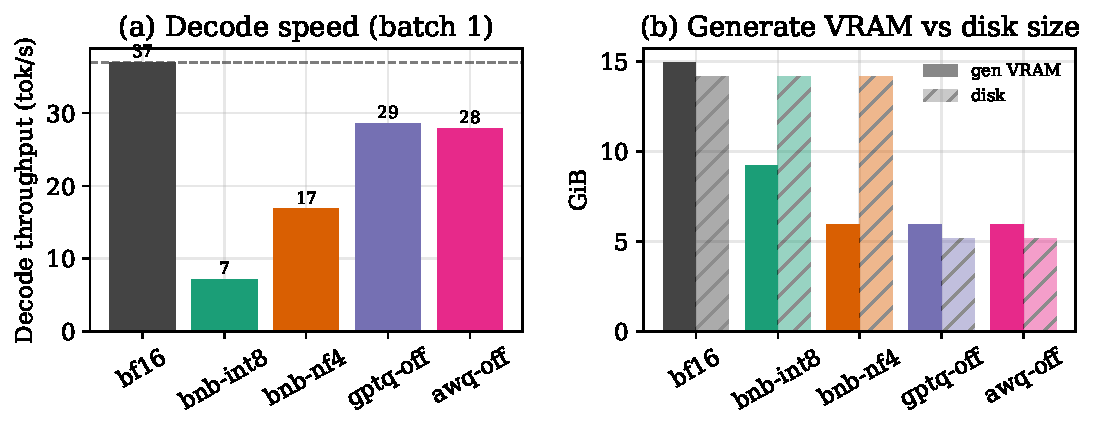
\includegraphics[width=0.99\linewidth]{fig_efficiency.pdf}
\caption{(a) Decode throughput (dashed line = \texttt{bf16}). \texttt{bnb-int8}
is $5\times$ slower; only GPTQ/AWQ stay near baseline. (b) Generate VRAM vs.\
on-disk size: \texttt{bitsandbytes} variants shrink VRAM but not disk; GPTQ/AWQ
shrink both.}
\label{fig:eff}
\end{figure}

\subsection{The trade-off and a recommendation (RQ1)}

Figure~\ref{fig:tradeoff} places all variants in the quality--speed--memory
space. The Pareto picture is unambiguous: \texttt{bf16} buys top speed at the
highest memory; \texttt{bnb-int8} is dominated (slow and disk-heavy);
\texttt{bnb-nf4} trades speed for memory; and \textbf{GPTQ/AWQ sit at the
sweet spot}---half the memory of NF4's disk footprint, the largest batch, and
${\sim}75\%$ of baseline decode speed for a ${\sim}1.5$\,pt MMLU cost. \emph{Our
recommendation under limited VRAM is an official GPTQ or AWQ checkpoint};
\texttt{NF4} is the best fallback when no pre-quantized checkpoint exists (it
needs only the base weights), and \texttt{LLM.int8()} is hard to recommend on
this hardware.

\begin{figure}[H]
\centering
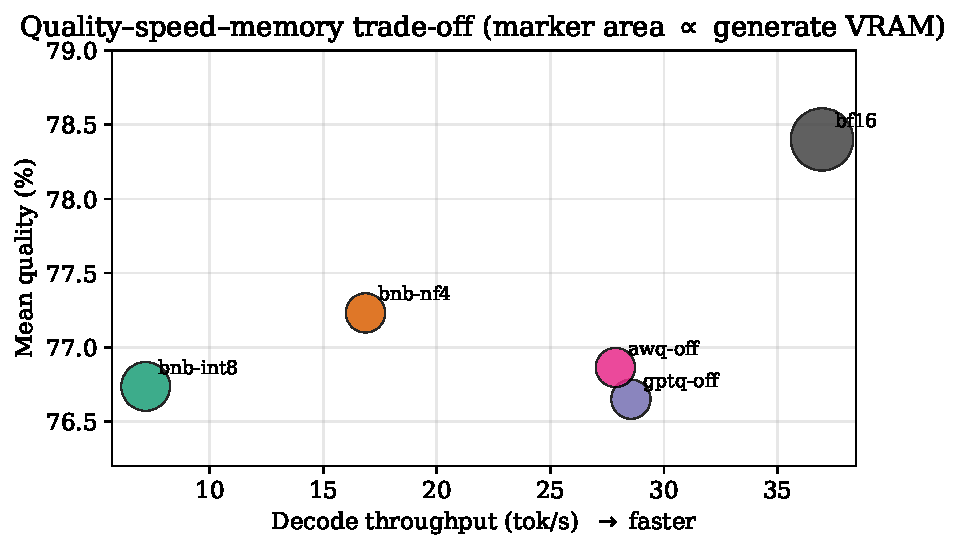
\includegraphics[width=0.74\linewidth]{fig_tradeoff.pdf}
\caption{Quality--speed--memory trade-off. Up-and-right is better (higher MMLU,
faster decode); smaller markers use less generate VRAM. GPTQ/AWQ dominate the
high-speed/low-memory corner; \texttt{bnb-int8} is Pareto-dominated.}
\label{fig:tradeoff}
\end{figure}

\section{Extensions}

We implemented all five catalogued extensions as a gated, separate code layer
(\texttt{qquant.ext}) that reuses the core harness without touching it, and ran
the four that fit the GPU budget (Mistral-7B as a second model was skipped---it
would re-spend the entire compute budget). The total extension run cost under
\$1 of GPU time.

\paragraph{EXT-2: JudgeBench (does quantization degrade \emph{judging}?).}
We evaluate each variant as a pairwise judge on JudgeBench \citep{judgebench}
(objective-correctness pairs), scoring agreement with the gold label under
position-bias control (both A/B orders must agree). Figure~\ref{fig:judge} shows
that \textbf{quantization does not degrade judging}: the 4-bit variants are if
anything marginally \emph{better} (\texttt{awq} $19.5\%$, \texttt{nf4} $19.0\%$)
than \texttt{bf16} ($12.0\%$). The absolute numbers are low because Qwen2.5-7B is
a weak, heavily position-biased judge on these hard pairs (only $22$--$33\%$ of
its verdicts are order-consistent)---a property of the base model, not of
quantization.

\paragraph{EXT-3: W8A8 / SmoothQuant.} We self-quantized a W8A8 checkpoint
\citep{smoothquant} (per-channel int8 weights + int8 activations) from the same
C4 calibration set as our 4-bit self-quant recipes, using \texttt{llm-compressor}
\citep{llmcompressor}. The checkpoint is produced and loads natively, but two
findings emerged on the HF runtime: (i) \texttt{compressed-tensors}
\emph{decompresses} W8A8 to a \texttt{bf16}-resident tensor ($15.2$\,GiB in VRAM),
so it yields \emph{disk-only} savings and no inference-memory benefit; and (ii)
its \texttt{generate()} path is severely \emph{runtime-confounded} on sm\_89
(${\sim}4.5$\,s/iteration at $28\%$ GPU utilisation), so a full quality sweep is
impractical---the slowdown is itself the result. W8A8 is best understood as a
vLLM/kernel-path technique, not an HF-\texttt{generate} one.

\paragraph{EXT-4: Quantized KV cache.} Using the transformers v5 quantized cache
(\texttt{quanto}, int4), we measured peak generation VRAM at a 3072-token context
(Figure~\ref{fig:kvcache}). The int4 KV cache cuts the KV+activation transient
$0.63\!\to\!0.49$\,GiB ($-22\%$) but slows decode \textbf{$\mathbf{20\times}$}
($31.3\!\to\!1.52$~tok/s), because \texttt{quanto} dequantizes the cache on every
step. This is a stark, quantitative confirmation of the ``runtime-confounded
throughput'' caveat: a quantized KV cache trades a modest memory saving for a
catastrophic speed cost on the HF backend, and is only worthwhile with a
fused kernel path (e.g.\ KIVI \citep{kivi} or vLLM).

\paragraph{EXT-5: QLoRA recovery (RQ4).} We verified the full QLoRA
\citep{qlora,lora} recovery pipeline end-to-end: a LoRA adapter (rank 16) trained
on the frozen NF4 base over \emph{general} instruction data---guarded by a
fail-fast check that the training corpus never overlaps the evaluation
benchmarks---and an adapter-aware load path. Training converged (loss $1.22$) and
the adapted model loads with the adapter active and generates coherently. A full
recovery \emph{measurement} (enough steps to move benchmark accuracy, then a
re-evaluation) is a longer campaign we leave to future work; here we contribute
the validated, contamination-safe machinery.

\begin{figure}[H]
\centering
\begin{subfigure}{0.52\linewidth}
  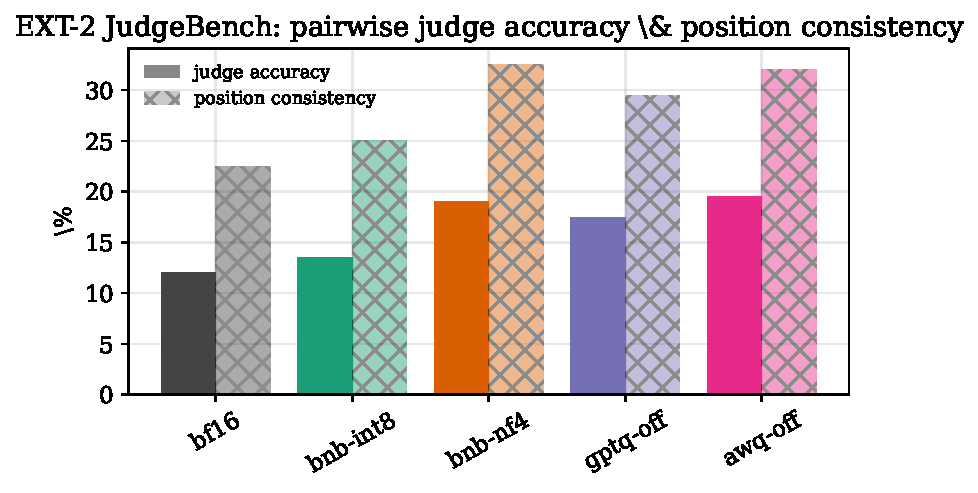
\includegraphics[width=\linewidth]{fig_judge.pdf}
  \caption{EXT-2 JudgeBench}
  \label{fig:judge}
\end{subfigure}\hfill
\begin{subfigure}{0.46\linewidth}
  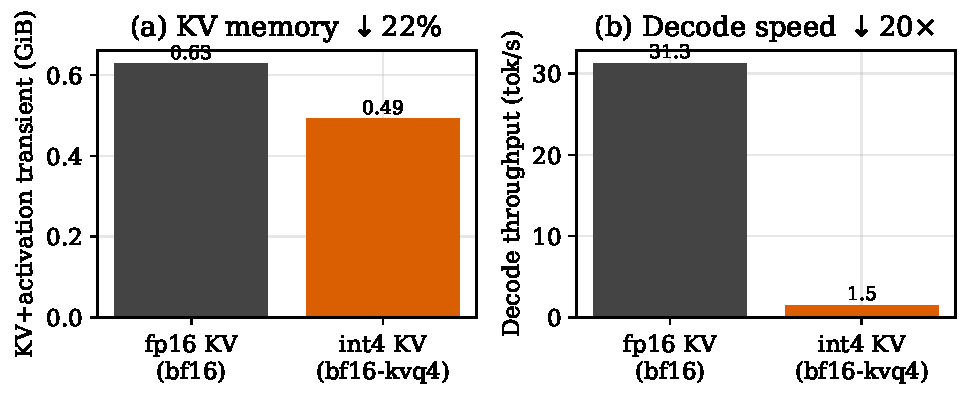
\includegraphics[width=\linewidth]{fig_kvcache.pdf}
  \caption{EXT-4 int4 KV cache}
  \label{fig:kvcache}
\end{subfigure}
\caption{Extension results. (a) Judge accuracy and position-consistency per
variant---quantization does not hurt judging. (b) int4 KV cache: $-22\%$ memory
transient but $20\times$ slower decode.}
\end{figure}

\section{Conclusion}

For a 7B-class instruction model on a single RTX~4090, \textbf{4-bit GPTQ/AWQ are
the best default under limited VRAM}: they cut disk by $2.7\times$ and generate
VRAM by $2.5\times$, double the feasible batch size, and keep decode within
$25\%$ of \texttt{bf16}, all for a graceful ${\sim}1.5$\,pt MMLU cost
(\textbf{RQ1}). Capability degradation is uneven---coding (HumanEval) is the most
sensitive, knowledge and math the least (\textbf{RQ2}). Most importantly,
\textbf{quantization is a memory technique, not a speed one} (\textbf{RQ3}):
\texttt{LLM.int8()} is $5\times$ \emph{slower} than \texttt{bf16} and saves no
disk, \texttt{NF4} saves memory while still decoding below baseline, and only the
calibrated 4-bit kernels (GPTQ/AWQ) deliver memory savings without a speed
penalty. Our extensions reinforce this: W8A8 and int4-KV-cache both ``work'' yet
are runtime-confounded on the HF backend, and quantization leaves judging quality
intact. The main limitations are single-seed evaluation and the runtime-confound
on the self-quant/KV paths, which a fused-kernel serving stack (vLLM) would
resolve; multi-seed runs, the second model (Mistral-7B \citep{mistral7b}), and a
full QLoRA recovery measurement (\textbf{RQ4}) are the natural next steps.

\section*{LLM Usage}
\small
In line with the course policy, we document our use of AI tools. The research
design (the variant matrix, the quality--memory--speed framing, and the
fairness/determinism protocol) is ours. We used an agentic coding assistant for
supporting engineering: the torch-free orchestration layer and vast.ai run
drivers, the evaluation/profiling harness scaffolding, the extension code layer,
and the figure- and table-generation scripts. Every quantitative claim in this
report was extracted programmatically from the committed result files and
cross-checked; agent-written code and prose were verified against the codebase
and the logged metrics before inclusion.
\normalsize

\bibliographystyle{plainnat}
\bibliography{references}

\newpage
\appendix
\section{Reproducibility and Full Efficiency Table}

\paragraph{Setup.} Single on-demand RTX~4090 (24\,GB, sm\_89) on vast.ai; torch
\texttt{2.12.1+cu126}, transformers \texttt{5.10.1}, \texttt{lm-eval}
(commit-pinned), \texttt{bitsandbytes 0.49.2}, \texttt{gptqmodel 7.1.0},
\texttt{compressed-tensors 0.17.1}. Greedy decoding; seeds fixed
(random/numpy/torch/few-shot). Quality and efficiency are profiled in separate
phases; each variant is loaded once. All result JSONs and the
extension/figure code are in the project repository; figures and tables in this
report are generated directly from those files.

\begin{table}[H]
\centering\small
\begin{tabular}{llccccc}
\toprule
Variant & Bucket & Prompt & Prefill & Decode & TTFT & E2E lat. \\
        &        & (tok)  & (tok/s) & (tok/s) & (s) & (s) \\
\midrule
\texttt{bf16}          & short/long & 128/4096 & 4141/9505 & 37.0/37.0 & 0.03/0.43 & 6.93/7.33 \\
\texttt{bnb-int8}      & short/long & 128/4096 & --/9220   & 7.2/7.2   & --        & -- \\
\texttt{bnb-nf4}       & short/long & 128/4096 & --/9196   & 16.9/16.9 & --        & -- \\
\texttt{gptq-official} & short/long & 128/4096 & --/9699   & 28.3/28.5 & --        & -- \\
\texttt{awq-official}  & short/long & 128/4096 & --/9615   & 28.0/27.9 & --        & -- \\
\bottomrule
\end{tabular}
\caption{Per-bucket throughput (selected fields; ``short/long'' = 128/4096-token
prompts). Decode is near-constant across prompt length, as expected for a
memory-bandwidth-bound phase. Full TTFT/latency per bucket are in the result
JSONs.}
\label{tab:eff-full}
\end{table}

\paragraph{Extension artifacts.} EXT-2 produced one JudgeBench cell per variant
($n{=}200$ pairs, position-bias controlled). EXT-3 produced an
$8.7$\,GiB W8A8 \texttt{compressed-tensors} checkpoint (per-channel int8 weights,
int8 activations) from the shared C4 calibration set. EXT-4 measured the int4
quantized KV cache at a 3072-token context. EXT-5 produced a rank-16 LoRA adapter
(general instruction data, contamination-guarded) and a verified adapter-attach
load path.

\end{document}
